% Source style adapted from https://tex.stackexchange.com/a/681912
\documentclass[tikz, margin=6mm]{standalone}
\usepackage[dvipsnames]{xcolor}
\usepackage{tikz}

\usetikzlibrary{fit, matrix, positioning, backgrounds, arrows.meta, calc}
\pgfdeclarelayer{background}
\pgfsetlayers{background,main}

\tikzset{
  every node/.style={font=\sffamily},
  % Row background highlight (no border, just fill)
  layerbg/.style={
    rounded corners=3pt,
    inner sep=3pt,
    draw=none,
  },
  % Left-column layer label box
  layerbox/.style={
    draw=white,
    rounded corners=3pt,
    minimum width=2.75cm,
    minimum height=1.12cm,
    text=white,
    align=center,
    font=\footnotesize\bfseries,
  },
  % Content item box
  itembox/.style={
    draw=white,
    rounded corners=3pt,
    minimum width=2.75cm,
    minimum height=1.12cm,
    text=white,
    align=center,
    font=\footnotesize,
  },
  % External tool box
  extbox/.style={
    draw=white,
    rounded corners=3pt,
    minimum width=3.35cm,
    minimum height=1.12cm,
    text=white,
    align=center,
    font=\footnotesize,
  },
  % Solid arrow: delegates-to (within framework, top-to-bottom)
  layerarrow/.style={
    line width=1.2pt,
    draw=black!55,
    -{Latex[length=2.7mm, width=2.0mm]},
  },
  % Dashed arrow: tool API call (adapter to external backend)
  toolcall/.style={
    line width=1.0pt,
    draw=black!50,
    dashed,
    -{Latex[length=2.4mm, width=1.8mm]},
    shorten >=2pt,
  },
}

\begin{document}
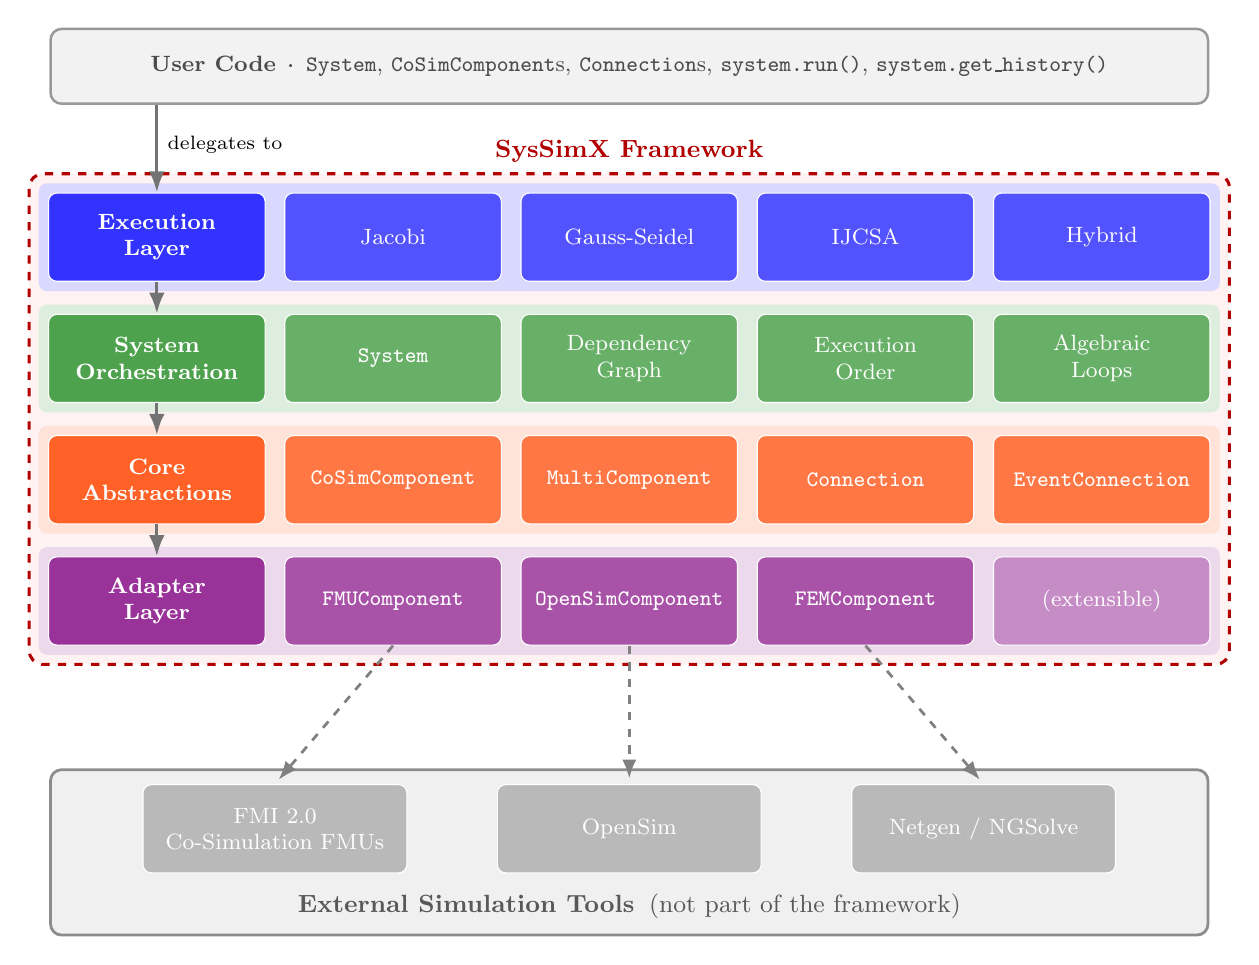
\begin{tikzpicture}

  % ---------------------------------------------------------------------------
  % Framework background matrix  (4 rows × 5 cols)
  %   Rows top-to-bottom: Execution | Orchestration | Core | Adapter
  %   Cols: Label | Item | Item | Item | Item
  % Row sep is kept wide enough so inter-layer arrows are visible.
  % ---------------------------------------------------------------------------
  \begin{pgfonlayer}{background}
    \matrix[
      fill=red!5,
      draw=red!70!black,
      dashed,
      line width=1.1pt,
      rounded corners=5pt,
      inner sep=7pt,
      row sep=0.42cm,
      column sep=0.25cm,
      nodes={minimum width=2.75cm, minimum height=1.12cm},
    ] (framework) {
      \node (r1c1) {}; & \node (r1c2) {}; & \node (r1c3) {};
        & \node (r1c4) {}; & \node (r1c5) {}; \\
      \node (r2c1) {}; & \node (r2c2) {}; & \node (r2c3) {};
        & \node (r2c4) {}; & \node (r2c5) {}; \\
      \node (r3c1) {}; & \node (r3c2) {}; & \node (r3c3) {};
        & \node (r3c4) {}; & \node (r3c5) {}; \\
      \node (r4c1) {}; & \node (r4c2) {}; & \node (r4c3) {};
        & \node (r4c4) {}; & \node (r4c5) {}; \\
    };

    % Horizontal layer backgrounds
    \node[layerbg, fill=Blue!15,        fit=(r1c1)(r1c5)] (bg1) {};
    \node[layerbg, fill=ForestGreen!15, fit=(r2c1)(r2c5)] (bg2) {};
    \node[layerbg, fill=OrangeRed!15,   fit=(r3c1)(r3c5)] (bg3) {};
    \node[layerbg, fill=Purple!15,      fit=(r4c1)(r4c5)] (bg4) {};
  \end{pgfonlayer}

  % Framework boundary label
  \node[
    anchor=north,
    fill=white,
    inner sep=2.5pt,
    font=\bfseries\small,
    text=red!70!black,
  ] at ([yshift=5mm]framework.north) {SysSimX Framework};

  % ---------------------------------------------------------------------------
  % Execution Layer  (row 1)
  % ---------------------------------------------------------------------------
  \node[layerbox, fill=Blue!80]  (exec_lbl) at (r1c1.center) {Execution\\Layer};
  \node[itembox,  fill=Blue!68]             at (r1c2.center) {Jacobi};
  \node[itembox,  fill=Blue!68]             at (r1c3.center) {Gauss-Seidel};
  \node[itembox,  fill=Blue!68]             at (r1c4.center) {IJCSA};
  \node[itembox,  fill=Blue!68]             at (r1c5.center) {Hybrid};

  % ---------------------------------------------------------------------------
  % System Orchestration  (row 2)
  % ---------------------------------------------------------------------------
  \node[layerbox, fill=ForestGreen!80] (orch_lbl) at (r2c1.center) {System\\Orchestration};
  \node[itembox,  fill=ForestGreen!68]            at (r2c2.center) {\texttt{System}};
  \node[itembox,  fill=ForestGreen!68]            at (r2c3.center) {Dependency\\Graph};
  \node[itembox,  fill=ForestGreen!68]            at (r2c4.center) {Execution\\Order};
  \node[itembox,  fill=ForestGreen!68]            at (r2c5.center) {Algebraic\\Loops};

  % ---------------------------------------------------------------------------
  % Core Abstractions  (row 3)
  % ---------------------------------------------------------------------------
  \node[layerbox, fill=OrangeRed!85]  (core_lbl) at (r3c1.center) {Core\\Abstractions};
  \node[itembox,  fill=OrangeRed!73]             at (r3c2.center) {\texttt{CoSimComponent}};
  \node[itembox,  fill=OrangeRed!73]             at (r3c3.center) {\texttt{MultiComponent}};
  \node[itembox,  fill=OrangeRed!73]             at (r3c4.center) {\texttt{Connection}};
  \node[itembox,  fill=OrangeRed!73]             at (r3c5.center) {\texttt{EventConnection}};

  % ---------------------------------------------------------------------------
  % Adapter Layer  (row 4)
  % ---------------------------------------------------------------------------
  \node[layerbox, fill=Purple!80] (adp_lbl) at (r4c1.center) {Adapter\\Layer};
  \node[itembox,  fill=Purple!68] (adp_fmu) at (r4c2.center) {\texttt{FMUComponent}};
  \node[itembox,  fill=Purple!68] (adp_osim)at (r4c3.center) {\texttt{OpenSimComponent}};
  \node[itembox,  fill=Purple!68] (adp_fem) at (r4c4.center) {\texttt{FEMComponent}};
  \node[itembox,  fill=Purple!45]            at (r4c5.center) {(extensible)};

  % ---------------------------------------------------------------------------
  % External Tools  —  outside framework boundary
  % ---------------------------------------------------------------------------
  \node[
    draw=black!45,
    rounded corners=4pt,
    line width=1pt,
    fill=Gray!12,
    minimum width=14.7cm,
    minimum height=2.1cm,
    anchor=north,
  ] (extrow) at ([yshift=-13mm]framework.south) {};

  \node[
    anchor=south,
    font=\bfseries\small,
    text=black!65,
  ] at ([yshift=1mm]extrow.south)
    {External Simulation Tools%
     \enspace\normalfont\small(not part of the framework)};

  \node[extbox, fill=Gray!55] (fmi)  at ([xshift=-4.5cm, yshift=3mm]extrow.center)
    {FMI 2.0\\Co-Simulation FMUs};
  \node[extbox, fill=Gray!55] (osim) at ([yshift=3mm]extrow.center)
    {OpenSim};
  \node[extbox, fill=Gray!55] (ngs)  at ([xshift=+4.5cm, yshift=3mm]extrow.center)
    {Netgen / NGSolve};

  % ---------------------------------------------------------------------------
  % User Code bar  —  above framework boundary
  % ---------------------------------------------------------------------------
  \coordinate (topcenter) at ($(r1c1.north)!0.5!(r1c5.north)$);

  \node[
    draw=black!40,
    rounded corners=4pt,
    fill=Gray!10,
    line width=0.9pt,
    minimum width=14.7cm,
    minimum height=0.95cm,
    font=\footnotesize,
    text=black!70,
    align=center,
    anchor=south,
  ] (userbar) at ([yshift=11mm]topcenter)
    {\textbf{User Code}\enspace·\enspace
     \texttt{System}, \texttt{CoSimComponent}s, \texttt{Connection}s,
     \texttt{system.run()}, \texttt{system.get\_history()}};

  % ---------------------------------------------------------------------------
  % Arrows  — solid: delegates-to  |  dashed: external API call
  % ---------------------------------------------------------------------------

  % 1. User Code → Execution Layer
  \draw[layerarrow]
    (userbar.south -| exec_lbl.north) -- node[pos=0.45, anchor=west, font=\scriptsize] {delegates to} (exec_lbl.north);

  % 2. Inter-layer delegation chain (left label column)
  \draw[layerarrow] (exec_lbl.south) -- (orch_lbl.north);
  \draw[layerarrow] (orch_lbl.south) -- (core_lbl.north);
  \draw[layerarrow] (core_lbl.south) -- (adp_lbl.north);

  % 3. Adapter → External Tools (dashed: crosses framework boundary)
  \draw[toolcall] (adp_fmu.south)  -- (fmi.north);
  \draw[toolcall] (adp_osim.south) -- (osim.north);
  \draw[toolcall] (adp_fem.south)  -- (ngs.north);

\end{tikzpicture}
\end{document}
